% Copyright 2021  Ed Bueler

\documentclass[xcolor={svgnames},
               hyperref={colorlinks,citecolor=DeepPink4,linkcolor=FireBrick,urlcolor=Maroon}]
               {beamer}

\mode<presentation>{
  \usetheme{Madrid}
  \usecolortheme{seagull}
  \setbeamercovered{transparent}
  \setbeamerfont{frametitle}{size=\large}
}

\setbeamercolor*{block title}{bg=red!10}
\setbeamercolor*{block body}{bg=red!5}

\usepackage[english]{babel}
\usepackage[latin1]{inputenc}
\usepackage{times}
\usepackage[T1]{fontenc}
% Or whatever. Note that the encoding and the font should match. If T1
% does not look nice, try deleting the line with the fontenc.

\usepackage{empheq}
\usepackage{xspace}
\usepackage{verbatim,fancyvrb}

\usepackage{tikz}
\usetikzlibrary{shapes,arrows.meta,decorations.markings,decorations.pathreplacing,fadings,positioning}


% If you wish to uncover everything in a step-wise fashion, uncomment
% the following command:
%\beamerdefaultoverlayspecification{<+->}

\newcommand{\ba}{\mathbf{a}}
\newcommand{\bb}{\mathbf{b}}
\newcommand{\bc}{\mathbf{c}}
\newcommand{\bbf}{\mathbf{f}}
\newcommand{\bg}{\mathbf{g}}
\newcommand{\bn}{\mathbf{n}}
\newcommand{\bq}{\mathbf{q}}
\newcommand{\br}{\mathbf{r}}
\newcommand{\bx}{\mathbf{x}}
\newcommand{\by}{\mathbf{y}}
\newcommand{\bv}{\mathbf{v}}
\newcommand{\bu}{\mathbf{u}}
\newcommand{\bw}{\mathbf{w}}

\newcommand{\bF}{\mathbf{F}}
\newcommand{\bG}{\mathbf{G}}
\newcommand{\bQ}{\mathbf{Q}}

\newcommand{\grad}{\nabla}
\newcommand{\Div}{\nabla\cdot}
\newcommand{\minmod}{\operatorname{minmod}}

\newcommand{\CC}{\mathbb{C}}
\newcommand{\RR}{\mathbb{R}}

\newcommand{\ddt}[1]{\ensuremath{\frac{\partial #1}{\partial t}}}
\newcommand{\ddx}[1]{\ensuremath{\frac{\partial #1}{\partial x}}}
\newcommand{\Matlab}{\textsc{Matlab}\xspace}
\newcommand{\Octave}{\textsc{Octave}\xspace}
\newcommand{\eps}{\epsilon}

\newcommand{\ip}[2]{\left<#1,#2\right>}

\newcommand{\xiphalf}{{x_{i+\frac{1}{2}}}}
\newcommand{\ximhalf}{{x_{i-\frac{1}{2}}}}
\newcommand{\Fiphalf}{{F_{i+\frac{1}{2}}}}
\newcommand{\Fimhalf}{{F_{i-\frac{1}{2}}}}
\newcommand{\Fiphalfn}{{F^n_{i+\frac{1}{2}}}}
\newcommand{\Fimhalfn}{{F^n_{i-\frac{1}{2}}}}

\newcommand{\trefcolumn}[1]{\begin{bmatrix} \phantom{x} \\ #1 \\ \phantom{x} \end{bmatrix}}
\newcommand{\trefmatrixtwo}[2]{\left[\begin{array}{c|c|c} & & \\ #1 & \dots & #2 \\ & & \end{array}\right]}
\newcommand{\trefmatrixthree}[3]{\left[\begin{array}{c|c|c|c} & & & \\ #1 & #2 & \dots & #3 \\ & & & \end{array}\right]}
\newcommand{\trefmatrixgroups}[4]{\left[\begin{array}{c|c|c|c|c|c} & & & & & \\ #1 & \dots & #2 & #3 & \dots & #4 \\ & & & & & \end{array}\right]}

\newcommand{\blocktwo}[4]{\left[\begin{array}{c|c} #1 & #2 \\ \hline #3 & #4 \end{array}\right]}

\newcommand{\bqed}{{\color{blue}\qed}}
\newcommand{\ds}{\displaystyle}

\newcommand\mynum[1]{{\renewcommand{\insertenumlabel}{#1}%
      \usebeamertemplate{enumerate item} \,}}


\title{Getting started with machine learning}

\subtitle{({applied math guy confronts artificial neural net})}

\author{Ed Bueler}

\institute[UAF]{MATH 692 Mathematics for Machine Learning \\ University of Alaska Fairbanks}

\date[Spring 2022]{13 January 2022}

%\titlegraphic{\begin{picture}(0,0)
%    \put(0,180){\makebox(0,0)[rt]{\includegraphics[width=4cm]{figs/software.png}}}
%  \end{picture}
%}

%% this nonsense needed to start section counter at 0; see
%% https://tex.stackexchange.com/questions/170222/change-the-numbering-in-beamers-table-of-content
\makeatletter
\patchcmd{\beamer@sectionintoc}
  {\ifnum\beamer@tempcount>0}
  {\ifnum\beamer@tempcount>-1}
  {}
  {}
%\beamer@tocsectionnumber=-1
\makeatother


\begin{document}
\beamertemplatenavigationsymbolsempty

\begin{frame}
  \maketitle
\end{frame}

\begin{frame}{today's talk}

\begin{itemize}
\item \alert{my topic:} how this $\downarrow$ neural network does a classification task

\medskip
\hspace{5mm} 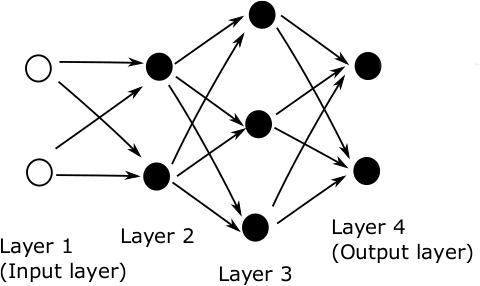
\includegraphics[height=25mm]{figs/network.png} \hfill 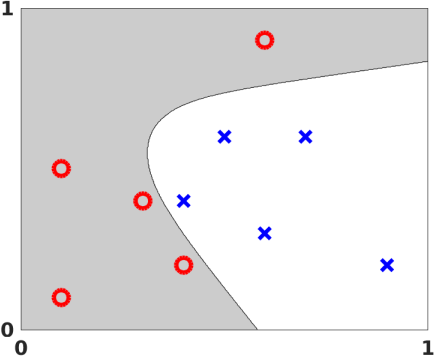
\includegraphics[height=23mm]{figs/classification} \hspace{10mm}

\medskip
\item it is an \alert{example} from this paper:

\medskip

HH19 \, $=$ \, 
\begin{minipage}[t]{0.75\textwidth} \footnotesize
C.~F.~Higham \& D.~J.~Higham (2019). \href{http://www.math.stonybrook.edu/~bishop/classes/math533.S21/MachineLearning/SIAMreview.pdf}{\emph{Deep learning: An introduction for applied mathematicians.}} SIAM Review, 61(4), 860-891
\end{minipage}

\normalsize
\medskip
\item \alert{goal for this talk:} know the meanings of

\medskip
\small
\qquad \begin{tabular}{ll}
\emph{artificial neuron} \qquad & \emph{activation function} \\
\emph{weight matrix} & \emph{bias vector} \\
\emph{back-propagation} & \emph{stochastic gradient method}
\end{tabular}

\normalsize
\medskip
    \begin{itemize}
    \item which standard mathematical concept(s) match these buzzwords?
    \end{itemize}
\end{itemize}
\end{frame}

\begin{frame}
  \frametitle{Outline}
  \tableofcontents[hideallsubsections]
\end{frame}

\section{logistics}

\begin{frame}{\emph{participant}-driven seminar}

\begin{itemize}
\item sign-up sheet!
\item webpages!
    \begin{itemize}
    \item \href{http://bueler.github.io/M692S22/index.html}{\texttt{bueler.github.io/M692S22}}
    \item \href{http://bueler.github.io/M692S22/resources.htm}{\texttt{bueler.github.io/M692S22/resources.htm}}
    \end{itemize}
\item in-person only or hybrid?
    \begin{itemize}
    \item is this classroom adequate?
    \end{itemize}
\item what will be the topics?
    \begin{itemize}
    \item are there out-of-bounds topics?
    \item who is volunteering to talk?
    \end{itemize}
\end{itemize}
\end{frame}


\section{a single artificial neuron}

\begin{frame}{fixme}

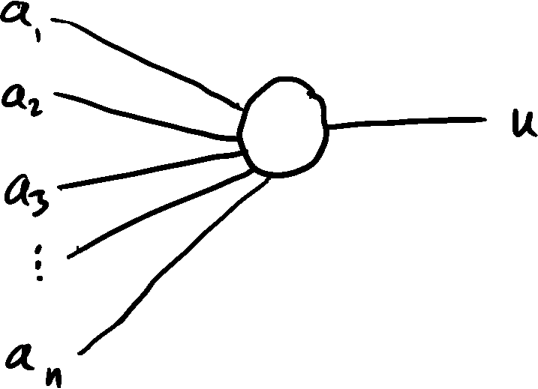
\includegraphics[height=25mm]{figs/single-neuron}

\begin{itemize}
\item latex
\item beamer
\end{itemize}
\end{frame}

\begin{frame}{fixme}

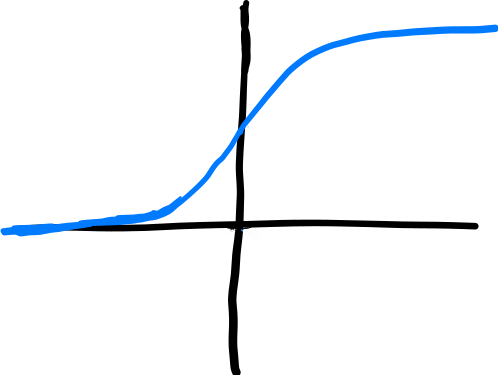
\includegraphics[height=25mm]{figs/sigmoid} \quad 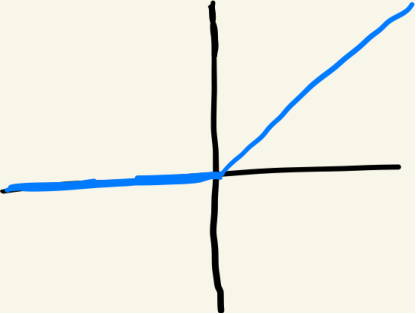
\includegraphics[height=25mm]{figs/relu}

\begin{itemize}
\item latex
\item beamer
\end{itemize}
\end{frame}


\section{forward through a neural net}

\begin{frame}{fixme}

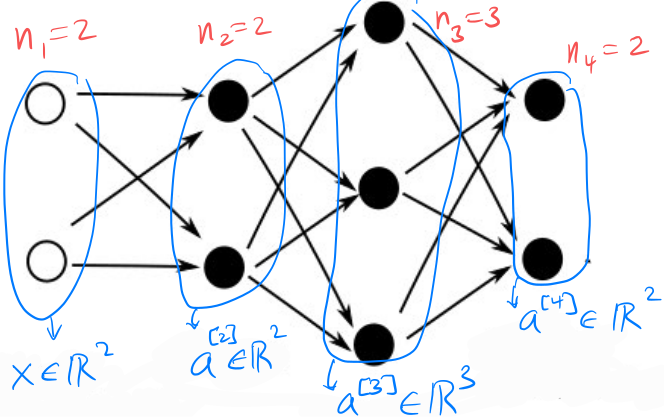
\includegraphics[height=25mm]{figs/state-notation}

\begin{itemize}
\item latex
\item beamer
\end{itemize}
\end{frame}

\begin{frame}{fixme}

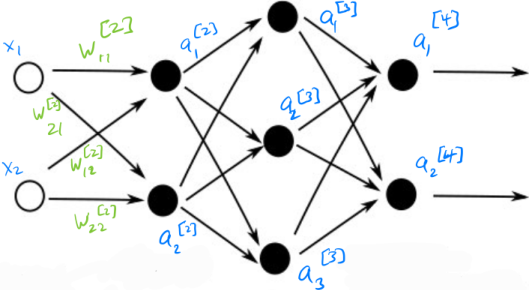
\includegraphics[height=25mm]{figs/weight-notation}

\begin{itemize}
\item latex
\item beamer
\end{itemize}
\end{frame}


\section{backward through a neural net}

\begin{frame}{fixme}

\begin{itemize}
\item latex
\item beamer
\end{itemize}
\end{frame}


\section{training is just optimization}

\begin{frame}{fixme}

\begin{itemize}
\item latex
\item beamer
\end{itemize}
\end{frame}


\section{running the codes yourself}

\begin{frame}{\emph{Matlab online} instructions: HH19 codes}

\begin{itemize}
\item as a UAF person you have access to Matlab online if you want it

\begin{center}
\href{https://matlab.mathworks.com/}{\texttt{matlab.mathworks.com}}
\end{center}

    \begin{itemize}
    \item I also use Octave
    \end{itemize}
\item 
\item beamer
\end{itemize}
\end{frame}


\begin{frame}{\emph{Matlab online} instructions: my versions of HH19 codes}

\begin{itemize}
\item FIXME
\item beamer
\end{itemize}
\end{frame}


\section{things that bother me}

\begin{frame}{fixme}

\begin{itemize}
\item latex
\item beamer
\end{itemize}
\end{frame}

\end{document}
